\section{Protocol Details}
\label{chp:protocol-details}
The target of \dprotocol is to provide a universal layer to simulate and synchronize the global state between various blockchains which support smart contracts. This universal layer is organized as a blockchain of \dprotocol nodes and each node contains four abstract components: storage component, transaction handler and simulator, native chain monitor and transaction finalizer.  Besides aggregator nodes, we also need to 
integrate native proxy contracts on native blockchains so that they can invoke transactions and update the local state accordingly.


\subsection{\dprotocol Node}
In a blockchain setting, we combine the finalizer, storage component, transaction handler and native chain monitor (everything except proxy contracts on native blockchains) together and equip it with an extra consensus component into a \dprotocol node. These distributed \dprotocol nodes form a blockchain that works together to synchronize and alter states between native blockchains. Each component in the node performs the following task:

\begin{enumerate}[leftmargin=*]
\item Chain Storage Component:
    \begin{itemize}
    \item store the global state.
    \item store the Merkle root hash of the whole state.
    \item store the valid voter list and the Merkle root hash of all voters.
    \end{itemize}
\item Transaction Handler and Simulator.
    \begin{itemize}
    \item order aggregator chain transactions under consensus.
    \item process transactions and update the whole state.
    \item emit transaction events (with execution order).
    \end{itemize}
\item Native Chain monitors:
    \begin{itemize}
    \item handle event emitted by invoke transaction of a bundled transaction.
    \item handle event emitted by revoke.
    \end{itemize}
\item Transaction Finalizer:
    \begin{itemize}
    \item calculate transaction execution proofs.
    \item calculate proofs of consensus.
    \item submit proofs to a guest chain for validation and finalization.
    \end{itemize}
\item Consensus component:
    \begin{itemize}
    \item perform consensus algorithm (voting block generator).
    \item calculate ZKP of the consensus algorithm.
    \item generate and prepare block.
    \end{itemize}
\end{enumerate}

Finally, proxy contract on the native-chain is also an important component of \dprotocol as it is used to maintain the partial state of a particular native chain by performing proof verification, state updating and processing the side effects of each transaction during the finalizing stage.  

As an example, suppose that we have two blockchains $C_{A}$ and $C_{B}$. Then our single \dprotocol involves the following entities (see Figure \ref{protocol-components})
\begin{figure}[!ht]
\centerline{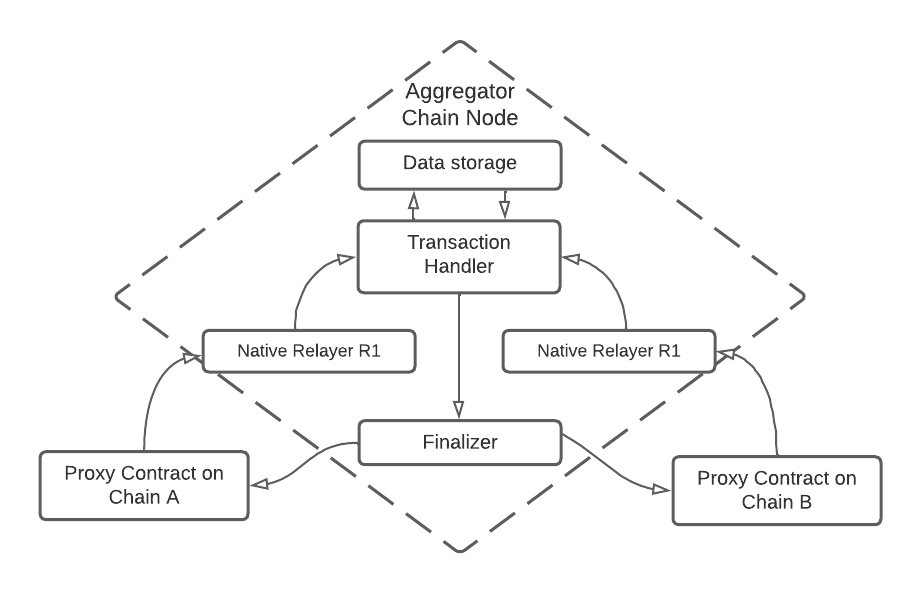
\includegraphics[scale=0.5]{components}}
\caption{Protocol components}
\label{protocol-components}
\end{figure}

%\noindent with each component performs the following functionalities:
%\begin{itemize}
%\item  Proxy smart contracts $\mathcal{A}$ and $\mathcal{B}$ on $C_A$ and $C_B$ (Trusted).
%\item  A transaction handler that handles and simulates transactions.
%\item  A storage component that tracks the global state.
%\item  Monitors $\mathcal{R}_A$ and $\mathcal{R}_B$ to monitor invoke (or revoke) transaction events for $C_A$ and $C_B$ and reports them to the transaction handler.
%\item  A finalizer that communicates with proxy contracts to finalize transactions.
%\end{itemize}
%\smallskip
%Moreover, 

\subsection{Transaction Lifecycle}
In \dprotocol the global state is compressed as a Merkle hash tree and pinned in all the guest chain proxy contracts. A bundled transaction $tx$ is a set of operations $tx_i^k: s_k \mapsto s_k'$. By defining how the local state $s_k$ of the application can be changed through $tx_i^k$, $tx$ can be treated as a function on the global state $s$. For a transaction to be successfully executed in \dprotocol, it undergoes the following four stages: (see Figure \ref{transaction-fifecycle}).
\begin{figure}[!ht]
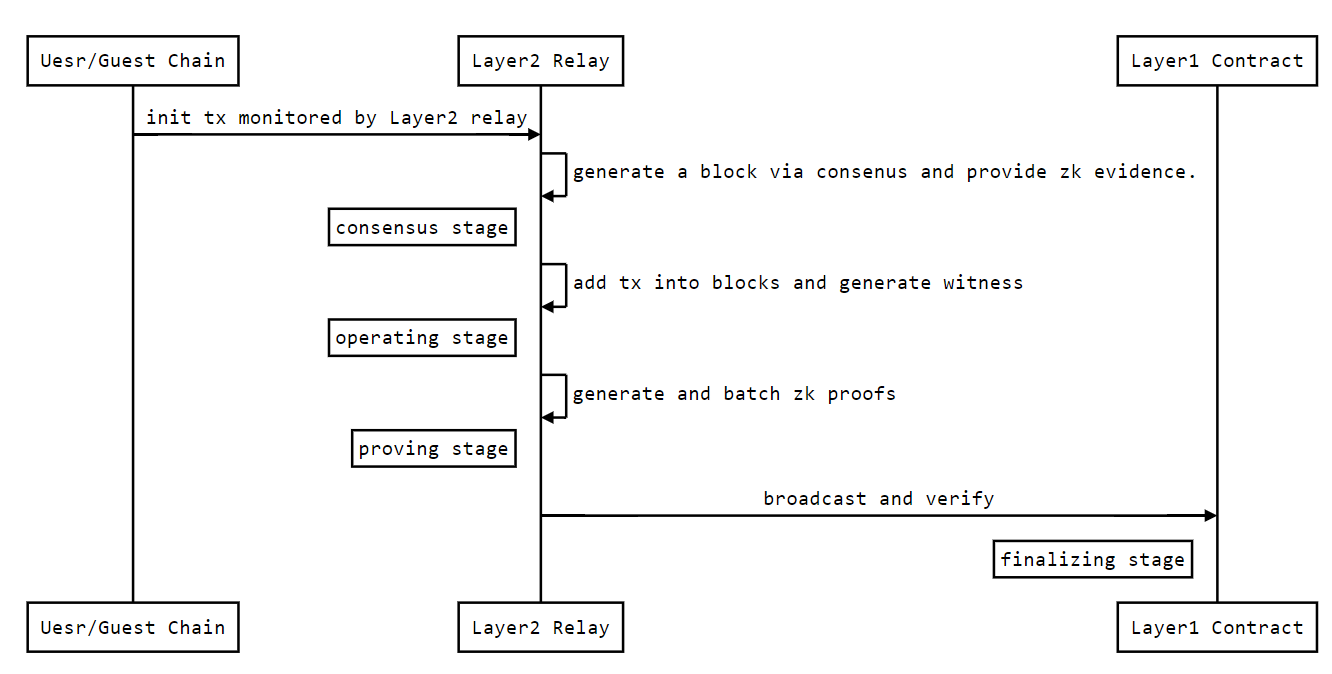
\includegraphics[scale=0.44]{consensus-sequence.png}
\caption{Transaction Life Cycle}
\label{transaction-fifecycle}
\end{figure}
\begin{enumerate}[leftmargin=*]
\item \emph{Consensus Stage:} As a decentralized protocol, a transaction will not get handled until it is collected in a block. Each block is produced by an elected node under a pre-defined consensus algorithm. A node that wins the consensus game needs to provide a ZK proof which will later be used as evidence to finalize all transactions within the block on the guest proxy contract.

\item \emph{Operating Stage:} At the operating stage, an operation is simulated on \dprotocol and changes the global state thus changing the Merkle root. During the simulation, all the information needed to create a ZKP for the simulation is prepared and stored. Since all transactions are handled sequentially regarding their order in a particular block, their proofs are stored in the same order so that they can be batched in the proving stage. 

\item \emph{Proving Stage:} After the operating stage, the finalizer will generate all the proofs for every transaction and compress proofs into a single ZKP proof. This proof is then appended after the transaction information in the block with an updated Merkle tree hash. 
\item \emph{Finalizing Stage:} Once the proof of batched operation sequence is generated by the finalizer, it will broadcast to various underlying blockchains. The blockchain needs to verify the proof, perform side-effects, and then emit acknowledge event to finalize the transaction.
\end{enumerate}

\subsection{Protocols in Each Stage}
\textbf{Consensus Stage.}
\label{consensus-stage}
A consensus algorithm is a common process in blockchain to achieve agreement on value or state among distributed nodes. A consensus algorithm is critical in systems that contain permissionless unreliable nodes. In \dprotocol we need a consensus algorithm to decide the following:

\begin{enumerate}[leftmargin=*]
\item Decide the order of the bundled cross-chain transactions.
\item Enroll and identify a valid node.
\item Vote a node to produce the next block and finalize the transactions in it. 
\end{enumerate}

In \dprotocol we use a modified PBFT \cite{castro1999practical} consensus algorithm between chain nodes to vote for a block generator. Recall that PBFT consensus consists of three phases: Pre-preparation, Preparation and Commit. At the Pre-preparation stage, the primary node is responsible for verifying the requests and generating corresponding pre-preparation messages. Then, in the preparation stage, the primary node will broadcast pre-preparation messages to all Replica nodes. After receiving the messages, Replica nodes will verify those pre-preparation messages and then broadcast a corresponding prepared message.

The final step in \dprotocol is carried out on native chains thus the results are not broadcast back to Replica nodes but broadcast to native chain nodes and verified there. Moreover, in addition to verifying that the results are correctly calculated, we also need to convince the guest chain that our generated blocks are produced under the consensus protocol as well. Usually, since the native chain does not attend the consensus algorithm in the aggregator-chain, it has the problem of checking whether the transaction results are reported from a fairly picked node. Thus we need to encode the consensus algorithm and its result into a zero-knowledge proof so that we can confirm the guest proxy contract that the block contains all transactions is generated legally. The consensus result together with its ZKP proof is stored in a newly generated block.

%as described as follows (see Figure \ref{block-layout}). 

%\begin{figure}[!ht]
%\begin{center}
%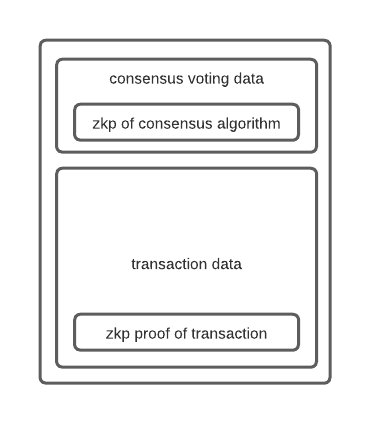
\includegraphics[scale=0.5]{block-data-layout}
%\end{center}
%\caption{Data layout of an aggregator block}
%\label{block-layout}
%\end{figure}

To satisfy all the above requirements, our modified PBFT approach still consists of three phases but each phase is slightly modified as described below.

First, at the pre-preparation stage, a node needs to be registered as a valid block generating candidate and broadcast the ZKP of the validation to other nodes. During the process of voting (preparation stage), each aggregator chain node in the consensus stage places a vote and sends a signature of the vote to their voting target. Suppose that two-thirds of the nodes in the system are honest then it follows that only one potential node will win the voting game and this particular node is authorized to produce a block.

Second, after a certain node gathers enough voting messages, instead of broadcasting the result, the winner node will calculate the ZKP of our consensus algorithm and put it into its generated block. This ZKP will later be used to convince the native blockchains that a batched transaction proof is sent from a legally voted node. Once the proof is attached to the newly generated block the winner node will start producing transactions (see Figure \ref{vote-sequence}).

\begin{figure}[!ht]
\begin{center}
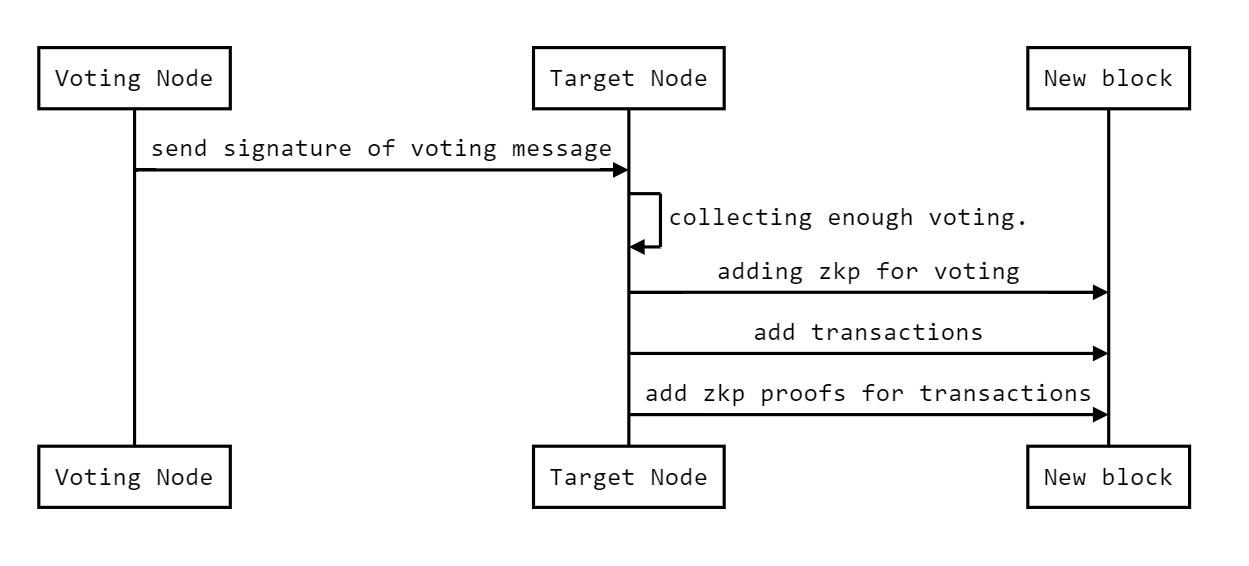
\includegraphics[scale=0.4]{vote-sequence.png}
\caption{Voting process during consensus}
\label{vote-sequence}
\end{center}
\end{figure}

In the end, the winner node will broadcast the generated block to the native blockchains. \dprotocol proxy contract on the native blockchain will verify and finalize this block and update its local state accordingly.

\dprotocol targets to build a permissionless chain that everyone can join the aggregator chain to helping to synchronize bundled cross-chain transactions. This means we need to provide a protocol to register and remove a valid voter. To achieve that, \dprotocol keeps a Merkle tree of all valid nodes by tracking their public keys as Merkle tree data nodes and anyone can register to be a valid node by registering itself as a new Merkle tree leaf. Also, for an aggregator node to vote for the next block producer, it has to prove the target it votes is a valid Merkle tree node (a registered valid node) first and then sign and send his voting ticket to the voted node. More precisely anyone can do the following:
\begin{enumerate}[leftmargin=*]
\item Register a node for voting:
    Node registration is an aggregator chain transaction that updates the Merkle tree of all valid voters on the aggregator chain and has the side effect of updating the Merkle tree root hash of nodes in the guest proxy contract. It is the responsibility of every aggregator node to keep the registration tree updated so that the root hash is consistent with the pinned hash in the proxy contract. 

\item Validate a voter:
    When a node receives voting from another node, it needs to validate that the sender is a valid voter. If the sender is an invalid node (eg, a malformed node without registration) then proof of sufficient voter will fail at the stage of finalizing thus wasting the computing source of the node who voted.

    Recall that all the valid voters are arranged in a Merkle tree whose root hash is pinned in the guest proxy contract. The voter needs to provide identity proof (in the form of ZK proof) to show that his public key (or voting address) is one of the Merkle tree leaf nodes.
    
    Once a node receives voting from voter $V$, it needs to verify the identity proof of $V$ first before it pushes it to the list of its supporters for the next block generation round.

\item Send a valid vote ticket:
    A voting ticket contains two parts, a signature, and validation proof. The signature is signed from the current block height together with the Merkle root hash of all valid voters. The validation proof is a zero-knowledge proof that proves that the voter is one of the valid voters. 
\end{enumerate}

\smallskip\noindent\textbf{Simulation Stage.}
After a node is voted as a block generator, it can start collecting transactions from various sources. In ZK Multi-Blockchain Aggregator, transactions are submitted to aggregator node, via three sources (see Figure \ref{simulation-stage}).

\begin{figure}[!ht]
\begin{center}
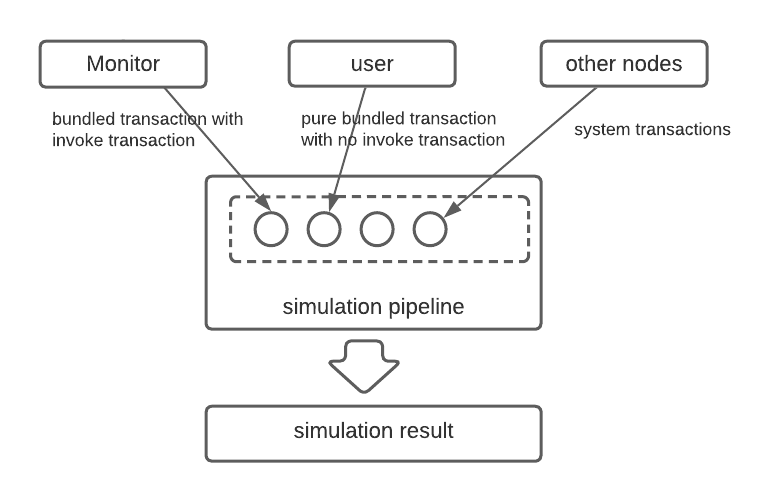
\includegraphics[scale=0.6]{simulation-pipeline.png}
\end{center}
\caption{Simulation stage}
\label{simulation-stage}
\end{figure}

\noindent\textit{1. The pure bundled transaction that does not contain an invoking transaction:} A pure bundled transaction is supposed to be sent directly to \dprotocol nodes and all its internal sub-transaction should either all succeed or fail. Notice that whether each sub-transaction will succeed (or all fail) can be determined via simulation in the aggregator node, the finalizer only finalizes succeeded transactions.

\noindent\textit{2. The bundled transaction that start with an invoking transaction}: This kind of bundled transaction is similar to the pure bundled transaction except that its first sub-transaction (and only the first sub-transaction) can not be simulated by the aggregator node. When handling this kind of transaction, the first transaction is executed on the native-block chain first and the monitor of the aggregator node monitors the result of the first transaction. If the first transaction is succeeded, the monitor submits the following transaction to the aggregator node. If not, the monitor submits a revoke transaction to the aggregator which will trigger a revoke of the invoking transaction just performed on the native-chain.

\noindent\textit{3. System transactions}: These kinds of transactions are submitted by aggregator nodes and it contains voting transaction, voter registration transaction, voter quit transaction, etc.

\smallskip\noindent\textbf{Proving Stage.}
As we discussed before, we simulate bundled transactions of the global state on the aggregator chain node and each bundled transaction is equivalent to a function $f: s \mapsto s'$. Since the global state is pinned on the native-chain by the Merkle hash root $h(s)$ of the state, a zero-knowledge proof of bundled transactions $tx$ is a proof that ensures the Merkle hash root of the result state $s' = f(s)$ is valid. 

\begin{figure}[!ht]
\begin{center}
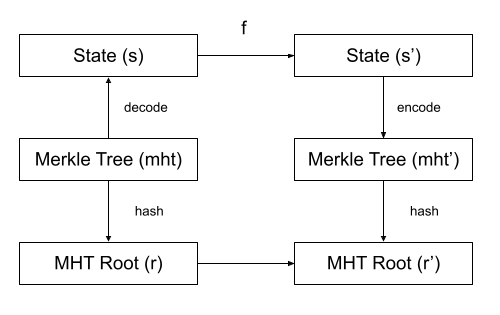
\includegraphics[scale=0.8]{circuit-state-refine}
\end{center}
\caption{State refine of transaction circuit}
\label{circuit-refine}
\end{figure}

For example (see Figure \ref{circuit-refine}), suppose that, before the transaction, state $s$ is encoded into the Merkle hash tree $mht$ which has root hash $r$ and after simulating the transaction the state changes to $s' = f(s)$. Also, suppose that this new state was stored in the aggregator chain storage in a format of updated Merkle tree $mht'$ whose new root hash is $r'$.
Then it follows that we need to create a zero-knowledge proof to show that the following constraints hold.
\[ constraints = \begin{cases}
    r = root(mht(s)) \\
    r' = root(mht(s'))\\
    mht(s') = mht(f(s))
\end{cases} \]
where the first two constraints are constraints about the state before and after the transaction and the last constraint is about the simulation of the function $f$.

%Moreover, $f$ can be treated as a sequence of leaf updates of the Merkle tree of state $s$. For each leaf update, suppose that $P_k = [p_0, p_1, p_2 \cdots p_n]$ is the MTI of an updated leaf of data $D_k$. It follows that to calculate the root hash after the modification of data of $D_k$, we need to calculate a new hash root at each level from $p_n$ to $p_0$ by the formula
%$$
%    H_k(p_k) = hash(H(p_{k+1}^0), H(p_{k+1}^1),\cdots) 
%$$
%where $a_i = p_{k+1}^{j}$ are nodes who have the same parent $p_k$ as $p_{k+1}$ \cite{liskov2005updatable}. A full transaction $tx$ is a data %transform function $f$ performed on multiple Merle leaf nodes. 

In \dprotocol node $f$ is defined as a combination of the following:

\begin{enumerate}[leftmargin=*]
\item Simple Merkle tree leaf update.
\item Predefined functions that have predefined ZKP circuits.
\item Cryptographic functions including signature functions and hash functions.
\end{enumerate}

\smallskip\noindent\textbf{Finalizing Stage.}
We know that a bundled transaction $tx$ is a state transformer over global state $s$ and is composed of a sequence of sub-transactions $tx^j_{k_j}$ on $C_{k_j}$. During the finalizing stage, \dprotocol mainly performs three things. First, it checks the ZKP of the consensus algorithm to make sure the block was generated by a valid block producer. Second, it checks the ZKP of the simulation of $tx$ so that the proxy contract can safely update the local state on $C_{k_j}$. Third, the proxy contract performs the side effects of $tx^j_{k_j}$ on $C_{k_j}$ (e.g., if a user would like to withdraw some asset from the aggregator chain to the guest chain, then during the finalizing procedure a transfer from the guest chain proxy contract to the target account of the withdrawal is executed).

\subsection{Guest Proxy Contract}
Guest Proxy Contract contains two parts: \emph{guest chain interface} and \emph{verification} interface (see Figure \ref{local-state}). Both of them manipulate the local state of guest chain. The guest chain interface includes invoke and revoke which allows guest chain users to invoke or revoke a message. The verification interface is called by \dprotocol node to finalize transactions.

\begin{figure}[!ht]
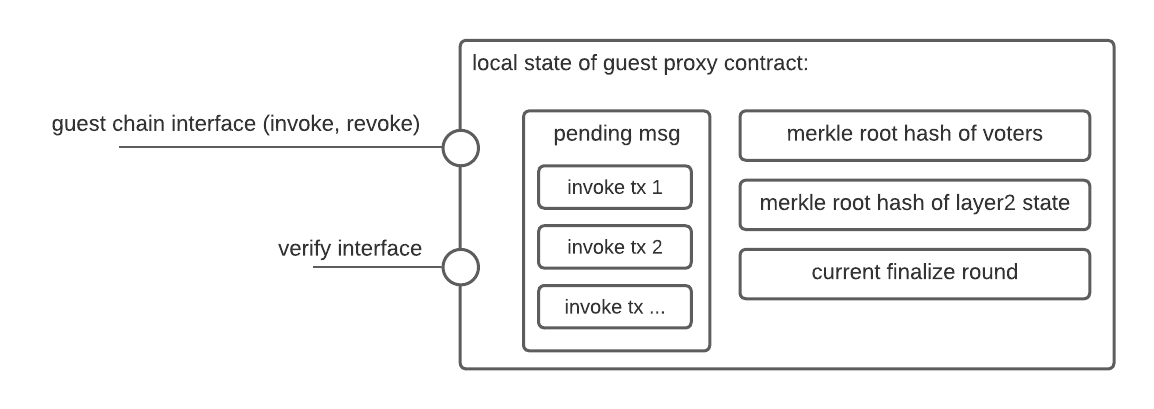
\includegraphics[scale=0.15]{proxy-local-state.png}
\caption{Local state of guest proxy contract}
\label{local-state}
\end{figure}

\subsubsection*{Guest chain interface.}
When a user invokes a {\bf guest chain interface}, the transaction info with the current block height ($h$) is recorded in the pending queue of the guest local state. The user who performed invoke transaction can revoke his invocation any time when the transaction remains in the pending queue after a fixed amount ($\delta_h$) of the block. This means \dprotocol nodes have to notice and handle this event and finalize this event within $\delta_h$ blocks.

%\begin{figure}[!ht]
%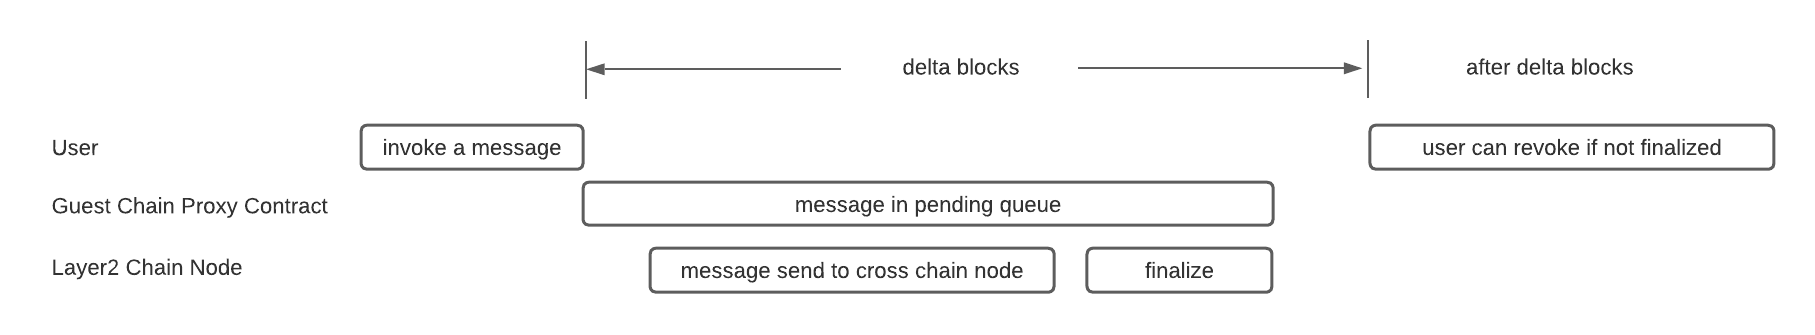
\includegraphics[scale=0.125]{whole-process}
%\caption{Time window for finalizing a block}
%\label{time-window-finalizing}
%\end{figure}

\subsubsection*{Verification Interface.}
The verification interface verifies the ZK-SNARK proof generated by the aggregator chain node (see Section 2.5).
\begin{figure}[!ht]
\begin{code}
function verify(
  uint256 l2account,
  uint256[] memory tx_data,
  uint256[] memory verify_data, // ZK proofs 
  uint256 vid,
  uint256 nonce,
  uint256 rid
)
\end{code}
\caption{Verification API in Native Blockchain}
\label{fig:verify-api}
\end{figure}

Recall that only the winner of the voting consensus of the current finalizing round ($rid$) is authorized to invoke the verification interface at round $rid$. It follows that the verification function (see Figure \ref{fig:verify-api}) first checks the voting proof to ensure that the sender is the winner of round $rid$ and then checks every transaction encoded in {\it tx\_data} is executed honestly via verifying the ZK proof encoded in {\it verify\_data}. If both check pass, the guest contract will perform all the side-effects of transactions on the guest chain accordingly (see Figure \ref{sideffects}).

\smallskip\noindent\emph{Types of transaction side-effects during finalization:}
\begin{itemize}[leftmargin=*]
\item \emph{Invoke:}
    An invocation $tx$ on the aggregator chain must be related to an invocation call on a guest contract, since every time a guest chain invocation will cause a record of pending invocation to be added to the pending list in the local state of the guest contract.
    Once a invoke $tx$ is verified, the side effect of that $tx$ is removing the invocation record in the pending invocation list.
    Once an invocation was removed from the pending invocation list, its sender loses the capability to withdraw it.

\item \emph{Callback:}
    The callback is a special transaction that is invoked through \dprotocol Node which tries to trigger a certain callback function from \dprotocol Chain to guest Chain.
    Once a callback $tx$ was verified, its side effect is to call a related guest contract API according to the $tx$ information.
    Withdraw is a special case of callback that calls the transfer API.

\item \emph{Generic Transaction:}
    All bundled transactions are simulated in aggregator nodes and the global state is pinned to the guest contract. So there is no other side-effect during the process of finalization for generic transactions.
\end{itemize}
\subsection{Guest Chain Monitor}
Guest chain monitor is responsible for monitoring guest chain events and notifying aggregator chain $tx$ handlers by forwarding them. The guest chain monitor needs to sign the event with its consensus ID. If a voted \dprotocol node failed to finalize its transactions in the guest chain proxy contract, then it either fails to calculate a correct ZKP proof of transactions and voting result or it does not pass the checks in the side-effect of invoking transactions in the guest contract. In the later case, the failed node could be a malicious node that provides invoking transactions that do not exist on the guest chain.  
\begin{figure}[!ht]
\begin{center}
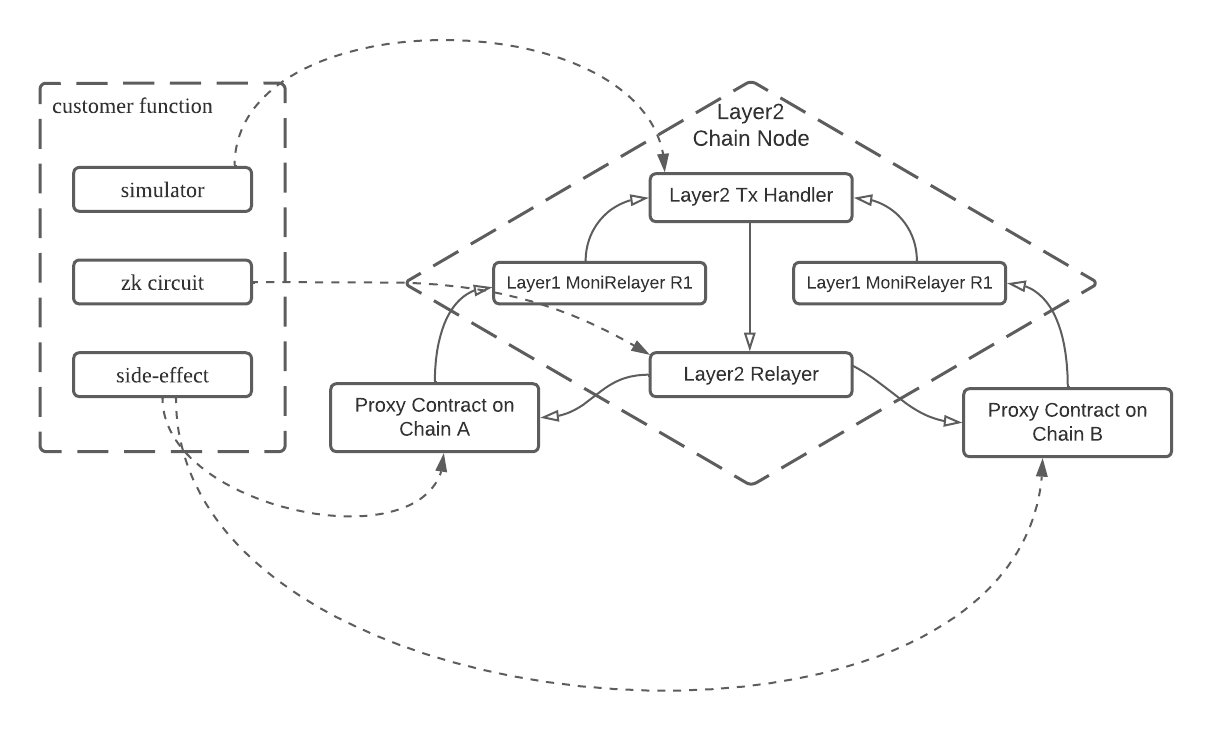
\includegraphics[scale=0.4]{side-effects}
\caption{Perform side effects of a bundled transaction}
\label{sideffects}
\end{center}
\end{figure}
